\documentclass[11pt]{article}

\usepackage[utf8]{inputenc}
\usepackage[T1]{fontenc}
\usepackage{times}
\usepackage{geometry}
\usepackage[english]{babel}
\usepackage{microtype}
\usepackage{pdfpages}
\usepackage{tocloft}
\usepackage{imakeidx}
\usepackage{dsfont}
\usepackage{titling}
\usepackage{parskip}
\usepackage{csquotes}
\usepackage{amsmath, amssymb, amsthm}
\setlength{\marginparwidth }{2.6cm}
\setlength{\headheight}{14.5pt}
\usepackage{todonotes, verbatim}
\usepackage{faktor}
\usepackage{fancyhdr}
\usepackage{pgfplots}
\usepackage{adjustbox}
\usepackage{tikz-cd}
\usetikzlibrary{decorations.pathmorphing}
\usepackage{multicol}

\usepackage{hyperref}
\usepackage{cleveref}


\graphicspath{{./images/}}
\pgfplotsset{compat=1.15}

\hypersetup{
colorlinks=true,
citecolor=[rgb]{0,0,0.8},
linkcolor=[rgb]{0,0,0.8},
}

\geometry{
    top=30mm, 
    bottom=30mm, 
    left=30mm, 
    right=30mm
}

%\theoremstyle{thmstyleone}
\newtheorem{theorem}{Theorem}
\newtheorem{corollary}{Corollary}
\newtheorem{proposition}{Proposition}
\newtheorem{lemma}{Lemma}

%\theoremstyle{thmstyletwo}
\newtheorem{example}{Example}
\newtheorem{remark}{Remark}
\newtheorem{question}{Question}
\newtheorem{acknowledgements}{Acknowledgements}

%\theoremstyle{thmstylethree}
\newtheorem{definition}{Definition}

\newcommand{\N}{\ensuremath{\mathbb{N}}}
\newcommand{\R}{\ensuremath{\mathbb{R}}}
\newcommand{\C}{\ensuremath{\mathcal{C}}}
\newcommand{\Z}{\ensuremath{\mathbb{Z}}} 
\newcommand{\Q}{\ensuremath{\mathbb{Q}}}
\newcommand{\A}{\ensuremath{A_{\infty}}}
\newcommand{\ls}{\text{cat}_{LS}}
\renewcommand{\ker}{\text{Ker}}
\newcommand{\ima}{\text{Im}}
\newcommand{\wH}{\widetilde{H}}
\newcommand{\wC}{\widetilde{C}}
\newcommand{\pir}{\pi^{\Q}}
\newcommand{\Hom}{\text{Hom}}
\newcommand{\Apl}{\text{A}_{PL}}
\DeclareMathOperator{\Tot}{Tot}

\cfoot{\thepage}

\tikzset{
%->,  
%>=stealth, 
node distance=2.3cm, 
every state/.style={thick, fill=gray!10},  
auto,
snake it/.style={decorate, decoration=snake}
}
\tikzstyle{every path}=[line width=0.8pt]




%%%%%%%%%%%%%%%%%%%%%%%%%%%%%%%%%%%%%%%%%%%%%%%%%%%%%%%%%%%%%%%%%%%%%%%%%%%%%%%%%%%%%% 


\title{Løsningsforslag til Equinor's promo-oppgaver}
\author{Torgeir Aamb\o}
\date{}

\begin{document}
\maketitle

\section*{Fra Konserthuset til Frognerparken}

Oppgaven er basert på konseptet om komplekse tall, som er en utvidelse av de vanlige tallene vi bruker til vanlig, altså alle heltall $1, 2, -4, 7$ etc, alle rasjonale tall $\frac{2}{3}, \frac{6}{17}$ etc, og alle reelle tall $\pi, \sqrt{2}, 0.99999...$, etc. Komplekse tall er todimensjonale, som gjør at vi kan bruke de til å beskrive posisjon på et kart. Det er i hovedsak to måter å beskrive et komplekst tall på, komplekse koordinater og polarkoordinater. Den førstnevnte er tall på formen $a+bi$ og den andre er tall på formen $r\mathrm{e}^{\phi i}$, hvor $a,b,r$ er reelle tall, $i$  er den imaginære enheten $\sqrt{-1}$ og $\phi$ er en vinkel oppgitt i radianer. I oppgaven er det oppgitt at vi står i posisjon $0+0i$, og at kongen bor ved $4.61\mathrm{e}^{\theta i}$, hvor $\theta=102.53^\circ$. 

Det første vi må gjøre er å uttrykke disse to posisjonene i samme type koordinater, og vi velger i dette forslaget å bruke komplekse koordinater. Vi ser at vinkelen til posisjonen til slottet er oppgitt i grader og ikke radianer, så vi konverterer først $102.53^\circ$ om til radianer ved å multiplisere med $\frac{\pi}{180}$. Vi får da $\phi = 1.78948608$ radianer. 

Vi kan konvertere fra polarkoordinater, $r\mathrm{e}^{\phi i}$, til komplekse koordinater, $a+bi$, ved å bruke følgende formler: 

\begin{itemize}
    \item $a = r\cdot \cos(\phi)$
    \item $b=r\cdot \sin(\phi)$
\end{itemize}

Gjør vi dette med kongens koordinater får vi $-1.00014 + 4.5002 i$, som vi kan avrunde til $-1+4.5i$. Dersom vi nå lar destinasjonen vår være $x+yi$ kan vi omformulere problemet vårt til 

$$
(x+yi)\cdot \frac{1}{49}(11-7i) = -1+4.5i,
$$

som vi kan løse for $x$ og $y$. Ved å gange ut venstre side av ligningen får vi 

$$
\frac{1}{49}(11x+7y)+\frac{1}{49}(11y-7x)i = -1+4.5i
$$

som vil si at vi må løse det følgende ligningssystem med to ukjente: 

\begin{itemize}
    \item $\frac{11}{49}x+\frac{7}{49}y = -1$
    \item $\frac{11}{49}y-\frac{7}{49}x = 4.5$
\end{itemize}

Vi kan enkelt løse dette ved å først løse den øverste ligningen for $x$, som gir $x=\frac{-49-7y}{11}$. Ved å sette dette utrykket inn for $x$ i den andre ligningen, samt å løse for $y$ får vi $y=12.25$. Denne verdien kan vi igjen sette inn i første ligning, som gir $x = 12.25$. Altså er posisjonen til destinasjonen vi skal til gitt som $12.25 + 12.25i$ i komplekse koordinater. 

Vi har nå nesten alt vi trenger for å finne destinasjonen vår, det siste vi trenger er et kart over Oslo. Vi legger inn posisjonen vår og posisjonen til slottet ved $(-1,4.5)$, markert med en rosa vektor. 

\begin{center}
    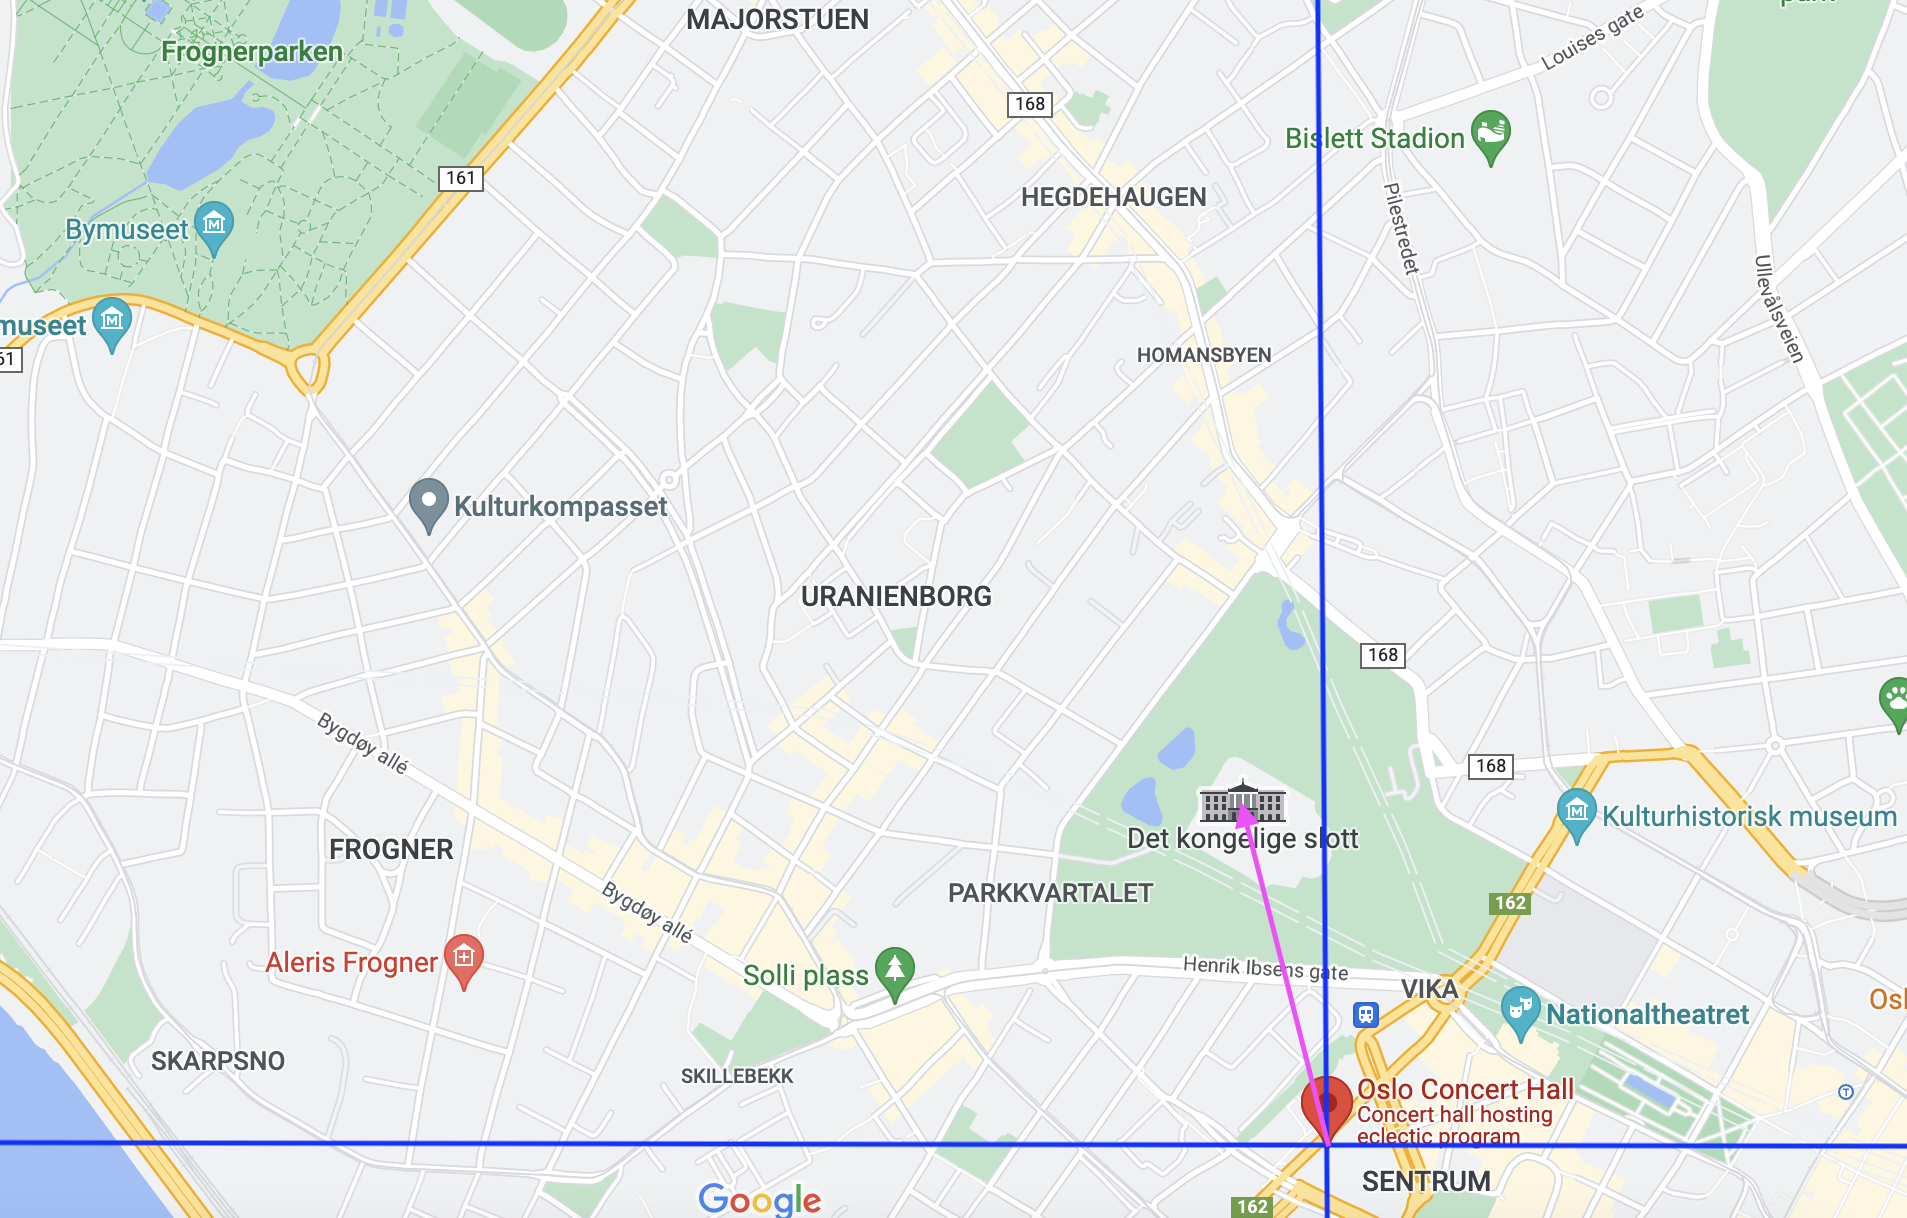
\includegraphics[width=\textwidth]{img/frogner.png}
\end{center}

Vi kan så bruke komponentene til denne vektoren til å finne destinasjonen vår. Vi får

\begin{center}
    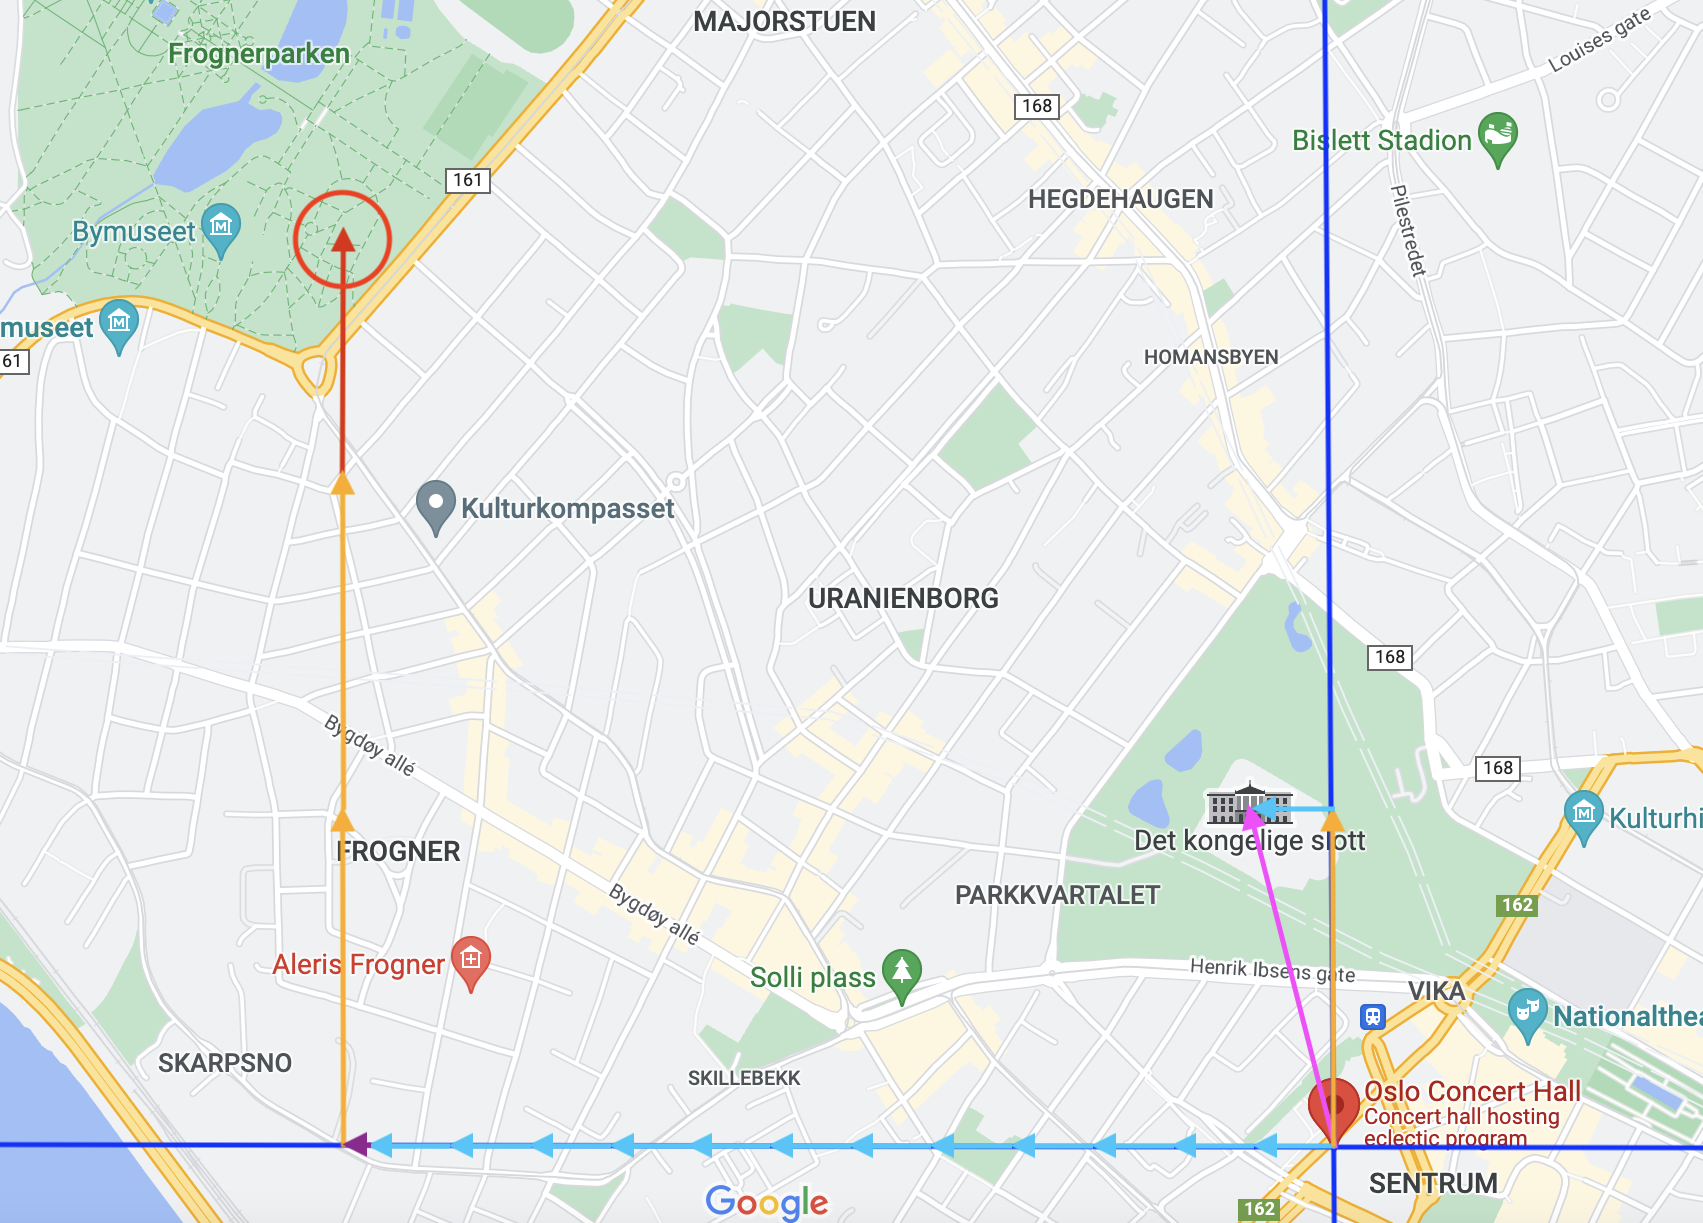
\includegraphics[width=\textwidth]{img/frogner_vec.png}
\end{center}

der de lyseblå vektorene har lengde $1$, de oransje har lengde $4.5$, den mørke blå har lengde $0.25$ og den røde har lengde $3.25$. Disse beskriver tilsammen posisjonen til destinasjonen vår $(12.25, 12.25)$. Dette viser at destinasjonen vår er Frognerparken!


\section*{Fra Rådhuset til Munchmuseet}

I matematikk liker man å vri å vende på konsepter man kanskje kjenner til allerede, for eksempel avstand. De fleste av oss har lært om Pytagoras’ læresetning i løpet av grunnskolen, som sier at $a^2+b^2=c^2$ for en rettvinklet trekant med kateter $a$ og $b$, og hypotenus $c$. Siden katetene står vinkelrett på hverandre kan vi se for oss at disse måler avstand i to unlike retninger.

Avstanden til punktet gitt av disse to katetene, er altså $c$, og vi kan finne denne avstanden ved å ta kvadratroten på begge sider av Pytagoras ligningen, altså 

$$
c = \sqrt{a^2+b^2}.
$$

Dette kan også skrives som $c = (a^2+b^2)^{\frac{1}{2}}$. For en matematiker ser dette veldig fristende ut å endre, ettersom vi kunne tenke oss å bytte ut tallet $2$ i ligningen med et hvilket som helst annet tall, for eksempel $(a^7+b^7)^{\frac{1}{7}}$ . For å sørge for at vi måler kun ‘positiv avstand’ tar vi absoluttverdien av $a$ og $b$ inne i dette utrykket. Dette kalles å måle avstand med $7$-norm, og i det generelle tilfellet $(|a|^p+|b|^p)^{\frac{1}{p}}$ kaller vi å måle avstand med $p$-norm. En litt mer vanlig måte å beskrive dette på er å ta en vektor $\vec x = (x_1, x_2)$ og skrive

$$
\Vert \vec x \Vert_p = (|x_1|^p+|x_2|^p)^{\frac{1}{p}} = \left(\sum_{i=1}^2 |x_i|^p\right)^{\frac{1}{p}}.
$$

Vi kan da se at måten vi måler avstand med til hverdags er bare et eksempel av alle disse måtene vi kunne ha gjort det på, det er nemlig $p$-normen med $p=2$. 

Kanskje tenker du at de andre måtene å måle avstand på bare er helt tullete — hvorfor skal vi bry oss om dette? Se for deg at du står midt i Manhattan i New York. Gatesystemet er et rutenett med to ulike retninger, og du vil bevege deg fra en side av et kvartal til motsatt side, altså rundt på baksiden. 

\begin{center}
    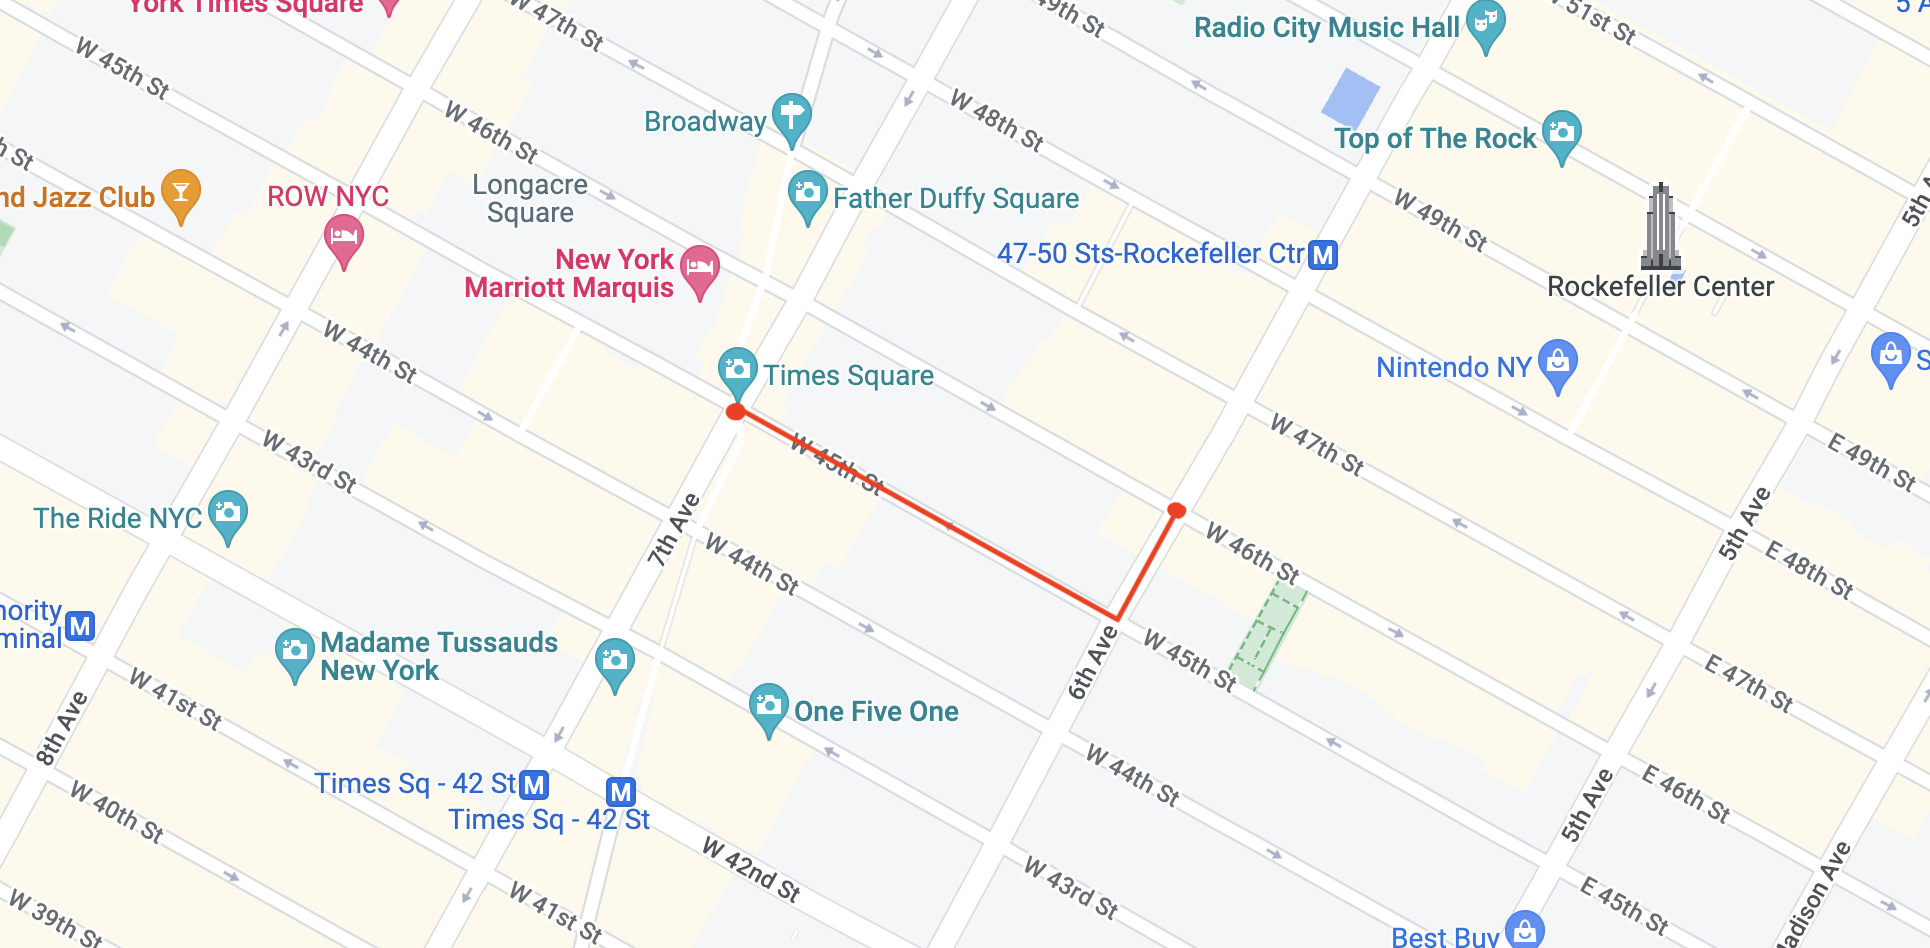
\includegraphics[width=\textwidth]{img/manhattan.png}
\end{center}

Måler vi avstand med den vanlige metoden får vi en rett linje som går diagonalt gjennom kvartalet, noe som ikke forteller oss hvor langt det faktisk er å gå, ettersom vi kun gan gå rundt. Dermed må vi måle avstand litt annerledes. Måten å gjøre dette på i Manhattan er å måle først strekningen i den ene retningen, og så plusse på strekningen i den andre retningen. Dette er nøyaktig det samme som å måle avstand med $1$-normen! Grunnet dette kalles $1$-normen ofte Taxi-normen, ettersom den beskriver hvor langt en taxi må kjøre i Manhattan for å komme seg til et sted. 

På den andre enden av spekteret har vi grenseverdien når $p\to \infty$. Denne normen kan også beskrives ved 

$$
\Vert \vec x \Vert_\infty = \max\{|x_1|, |x_2|\}.
$$

Nå har vi alt vi trenger for å løse oppgaven. Vi har oppgitt at vi befinner oss i $(0,0)$ og at destinasjonen vår er på land mot øst med $1$-norm avstand $\Vert \vec x \Vert_1 = |x_1|+|x_2| = 1.9\mathrm{km}$ og $\infty$-norm avstand $\Vert \vec x \Vert_\infty = \max\{|x_1|, |x_2|\}=1.25\mathrm{km}$. Dermed vet vi automatisk at enten $|x_1|=1.25$ eller $|x_2|=1.25$, noe som betyr at den andre må være $1.9-1.25 = 0.65$. Disse kan vi enkelt legge inn på et kart og se hvor vi ender opp. 

\begin{center}
    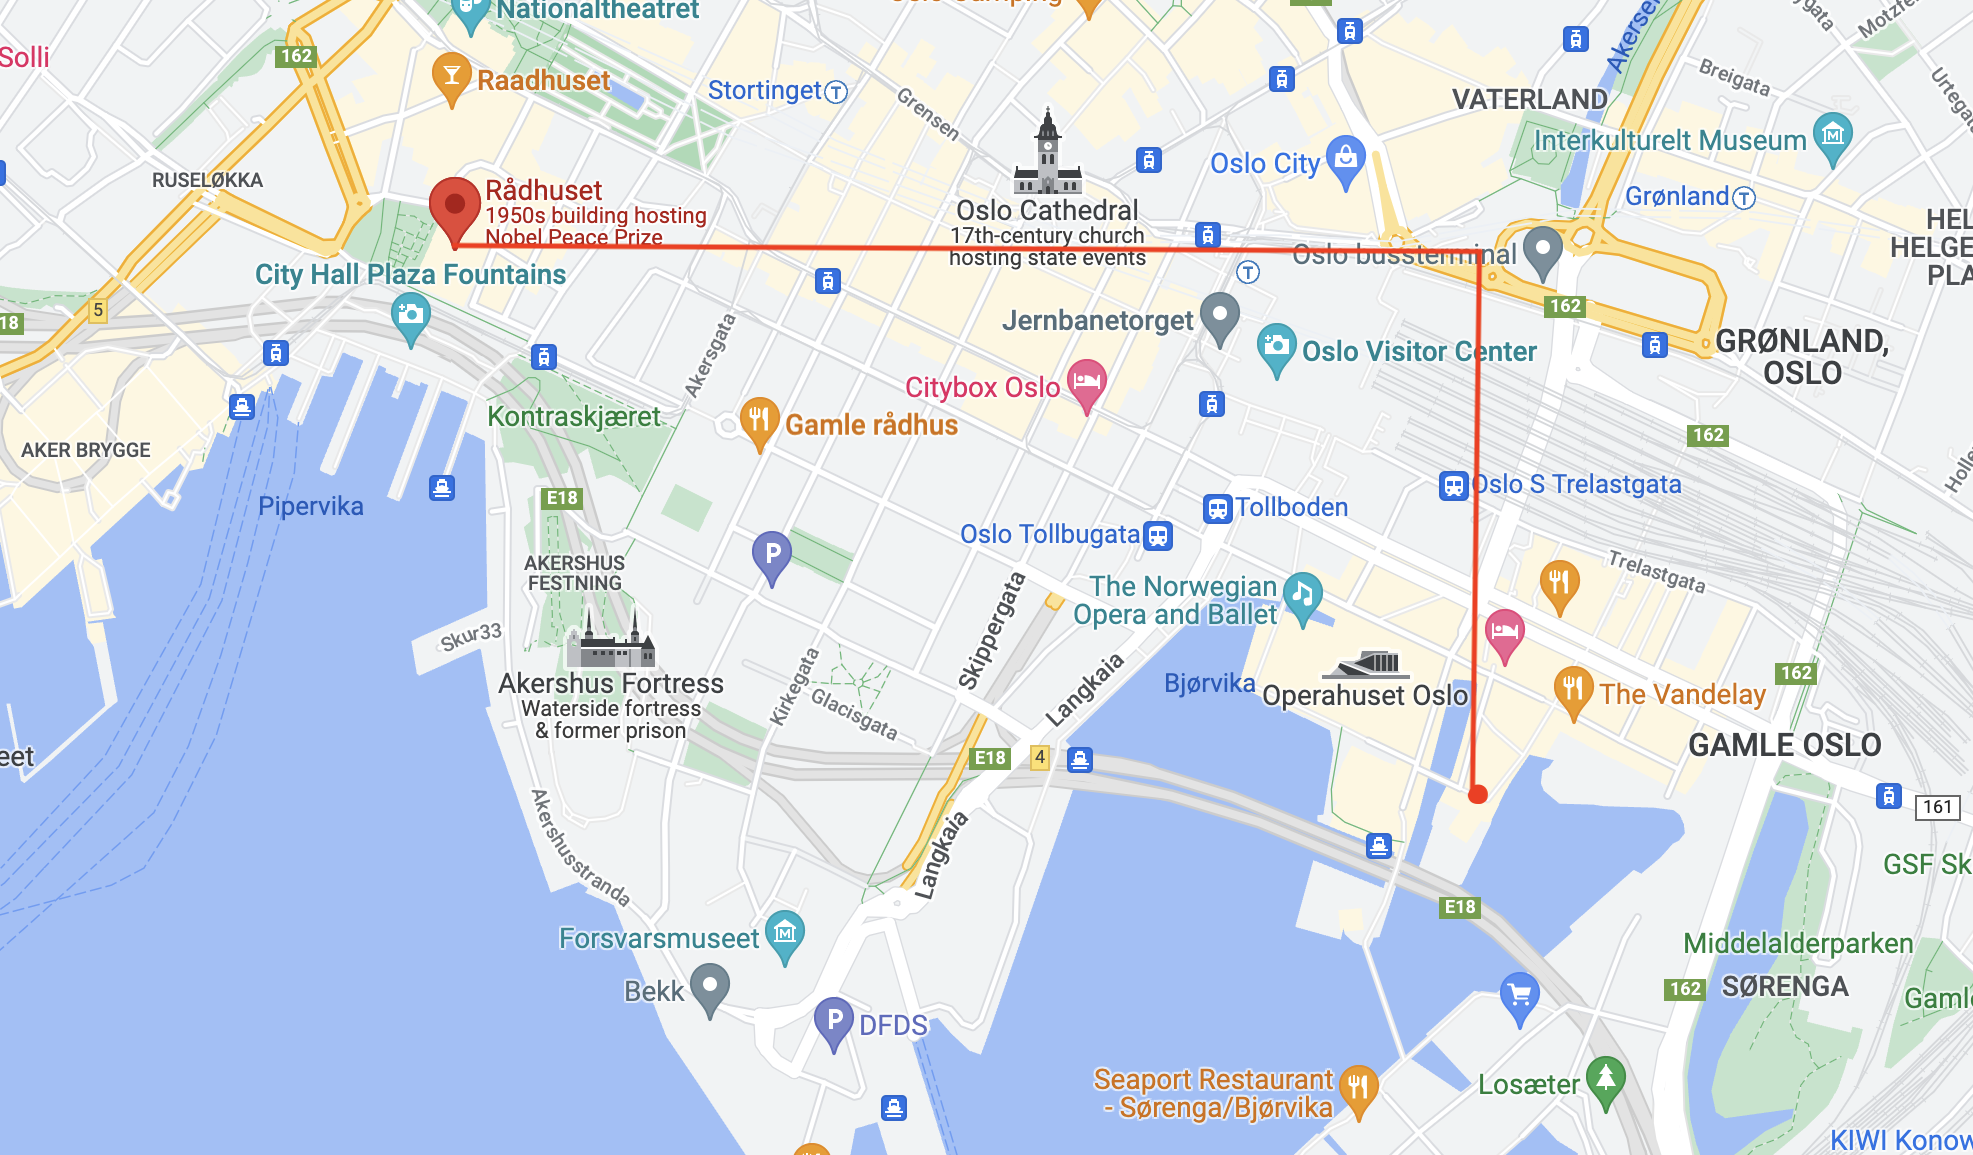
\includegraphics[width=\textwidth]{img/munch_2.png}
\end{center}

Vi ser at kun det ene punktet er på land, som betyr at det er dit vi skal. Ser vi på kartet er det nøyaktig Munch museet som er destinasjonen. 


\section*{Fra Pilestredet til Teknisk museeum}

Destinasjonen vår er er gitt ved en gateadresse, Kjelsåsveien $k$, og oppgaven vår er dermed å finne ut hva $k$ er. Vi har gitt at $k=p\cdot q$, hvor $(p,q)$  danner et tvillingprimtallspar, så la oss først liste opp noen av disse. Tvilling primtall er primtall som er kun $2$ heltall fra hverandre, altså at både $p$ og $p+2$ er primtall. Et eksempel er $3$ og $5$, som også er det første tvillingprimtallsparet. Merk at $2$ og $3$ ikke regnes som et tvillingprimtall. De første fem parene er $(3,5)$, $(5,7)$, $(11,13)$, $(17,19)$ og $(29,31)$. 

Den neste biten med informasjon vi får oppgitt er at $(p,q)$ er det $n$’te tvillingprimtallsparet. Så la oss nå prøve å finne ut hva $n$ kan være. Tallet $n$ skal være antall Platonske legemer i dimensjon $k$, noe som gjør at vi har et slags rekursivt definert problem. Men først, hva er en Platonsk legeme? Matematisk presist er det et konvekst legeme bestående av regulære like polyhedre, men dette kan mye bedre forklares ved å vise et eksempel: 

\begin{center}
    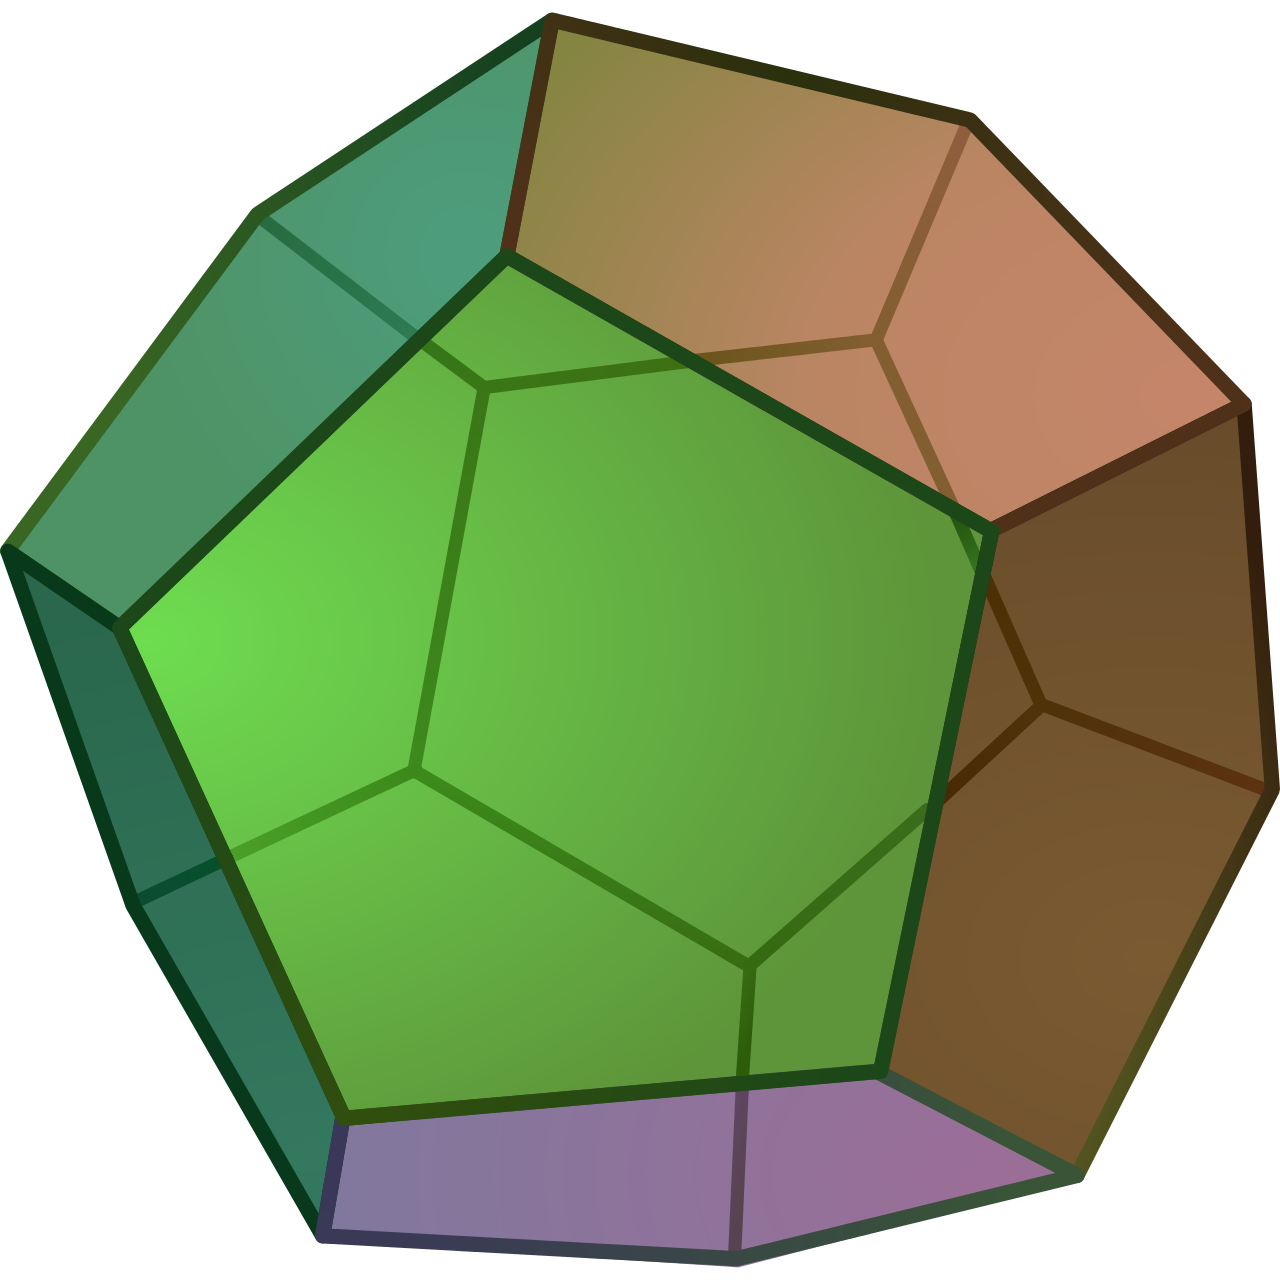
\includegraphics[height = 7cm]{img/Dodecahedron.png}    
\end{center}

Her ser vi at legemet består av av $12$ helt like femkanter, og at ingenting rart stikker ut noen sted. Dette er altså et Euklidsk legeme i dimensjon $3$. I dimension tre har vi fem slike legemer, som kalles for tetraederet,

\begin{center}
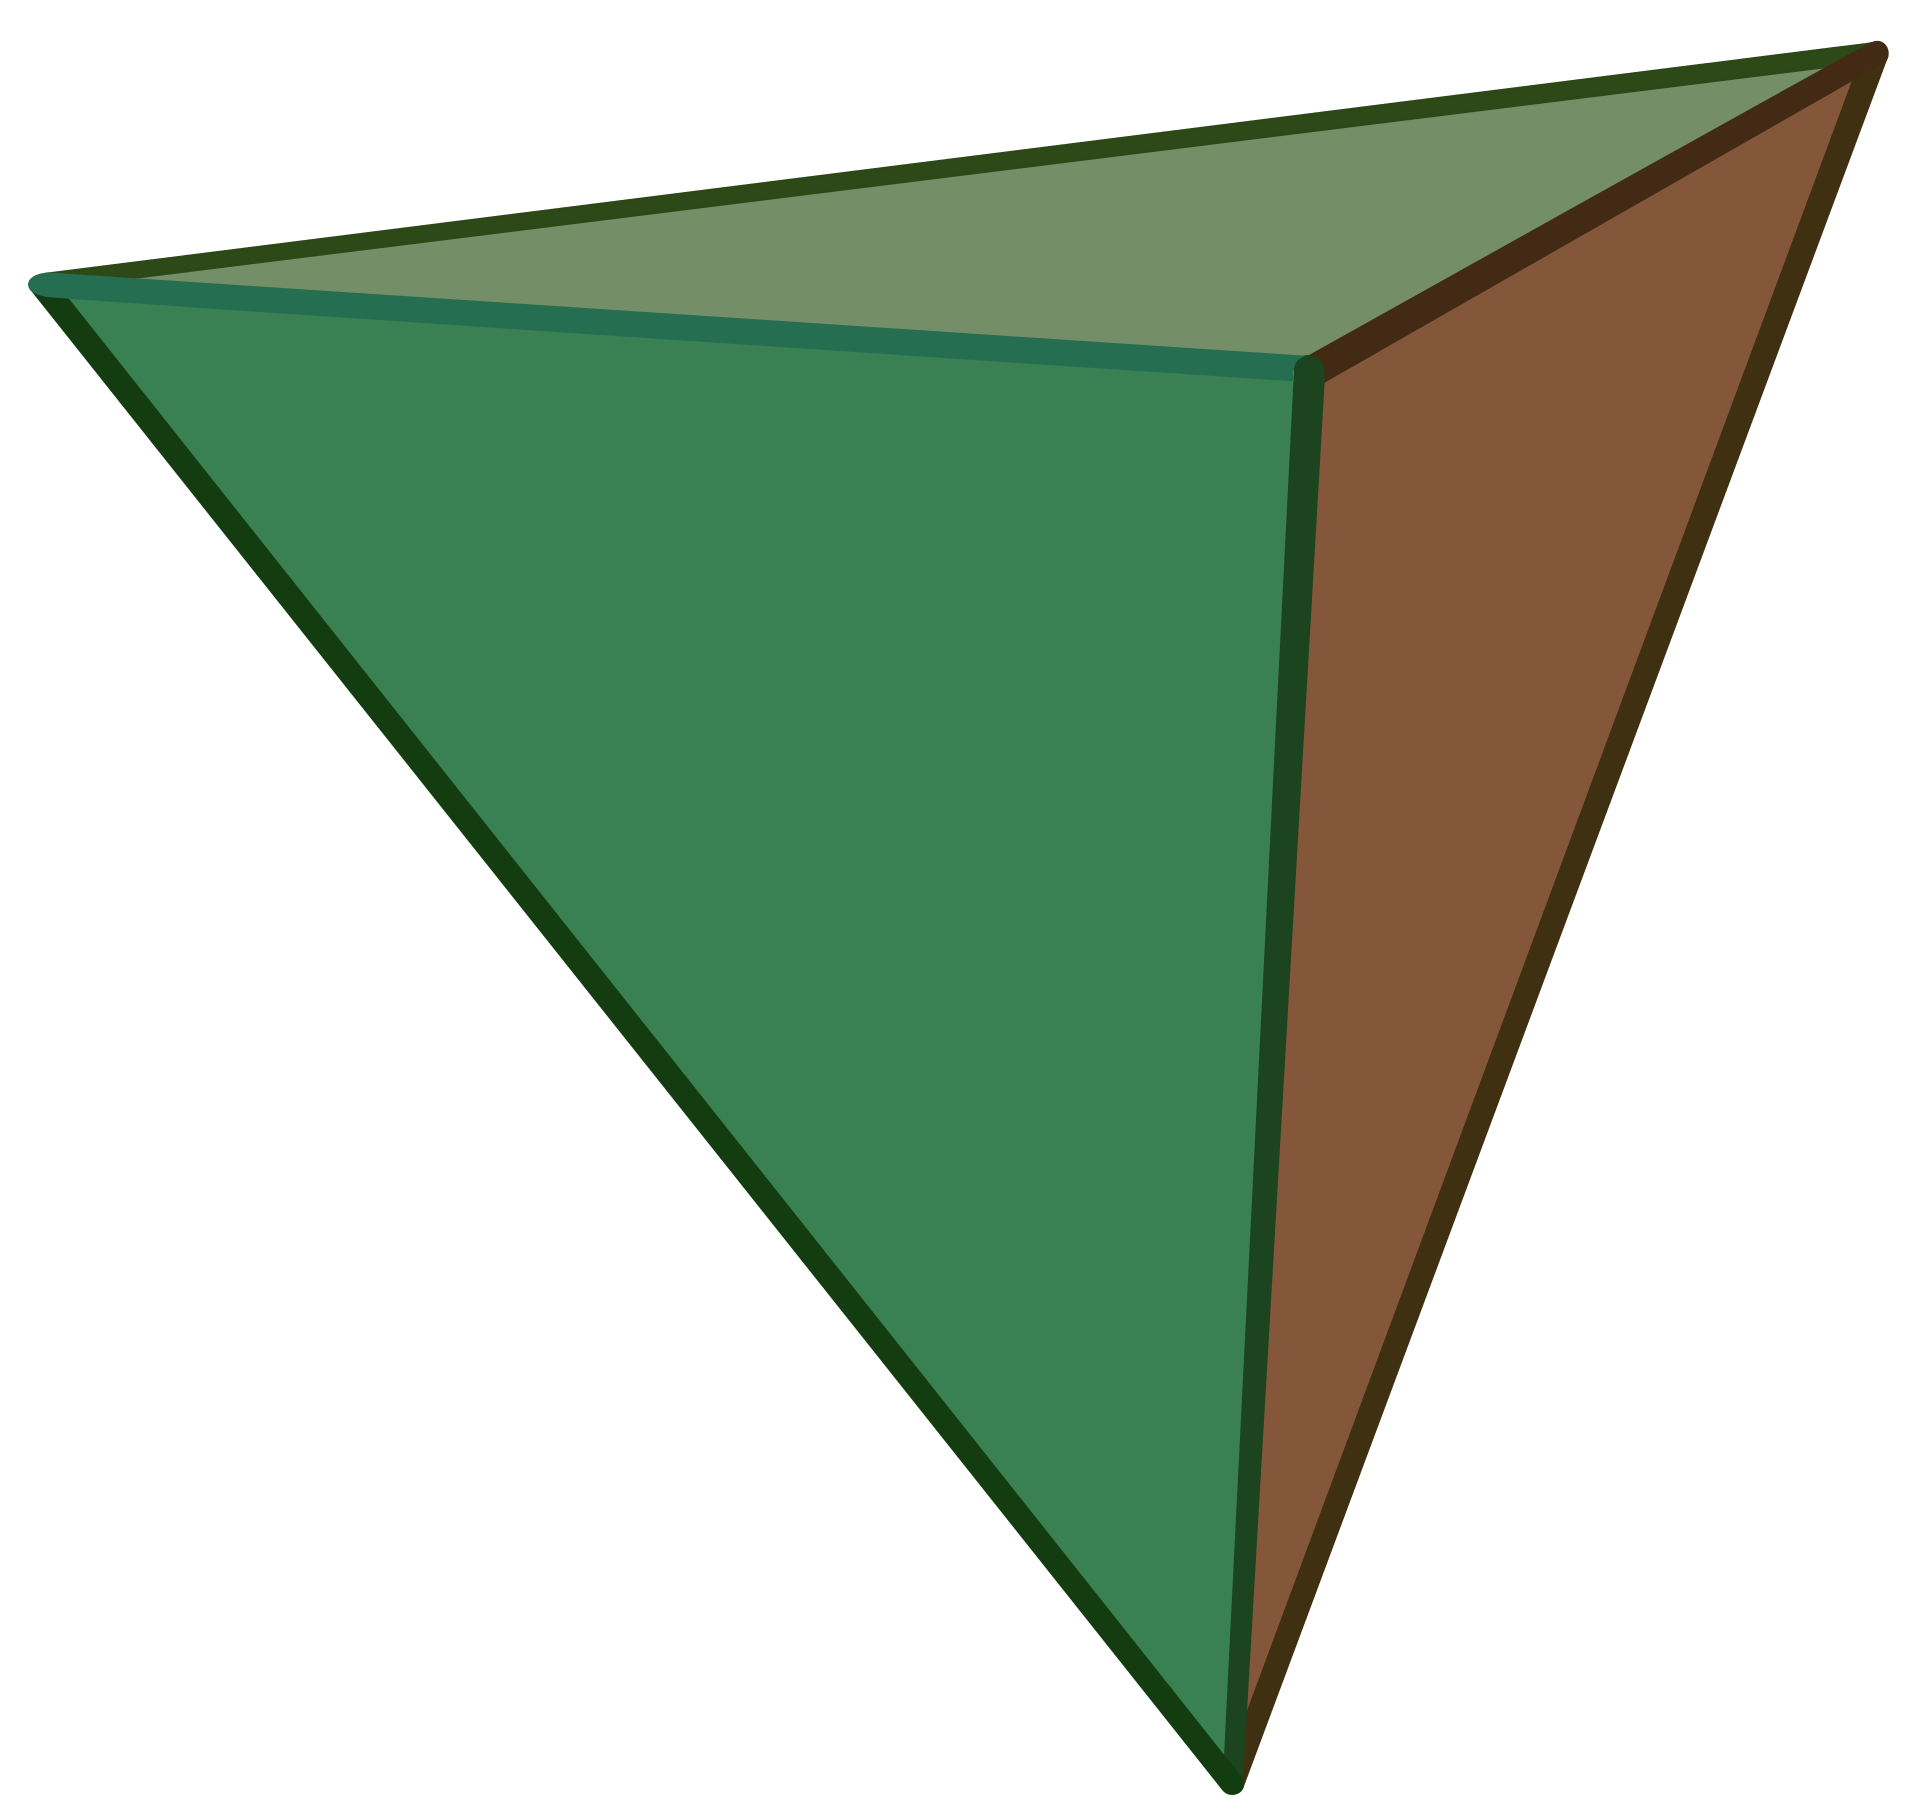
\includegraphics[height = 6cm]{img/Tetrahedron.png}
\end{center}

heksaederet, bedre kjent som en kube,

\begin{center}
    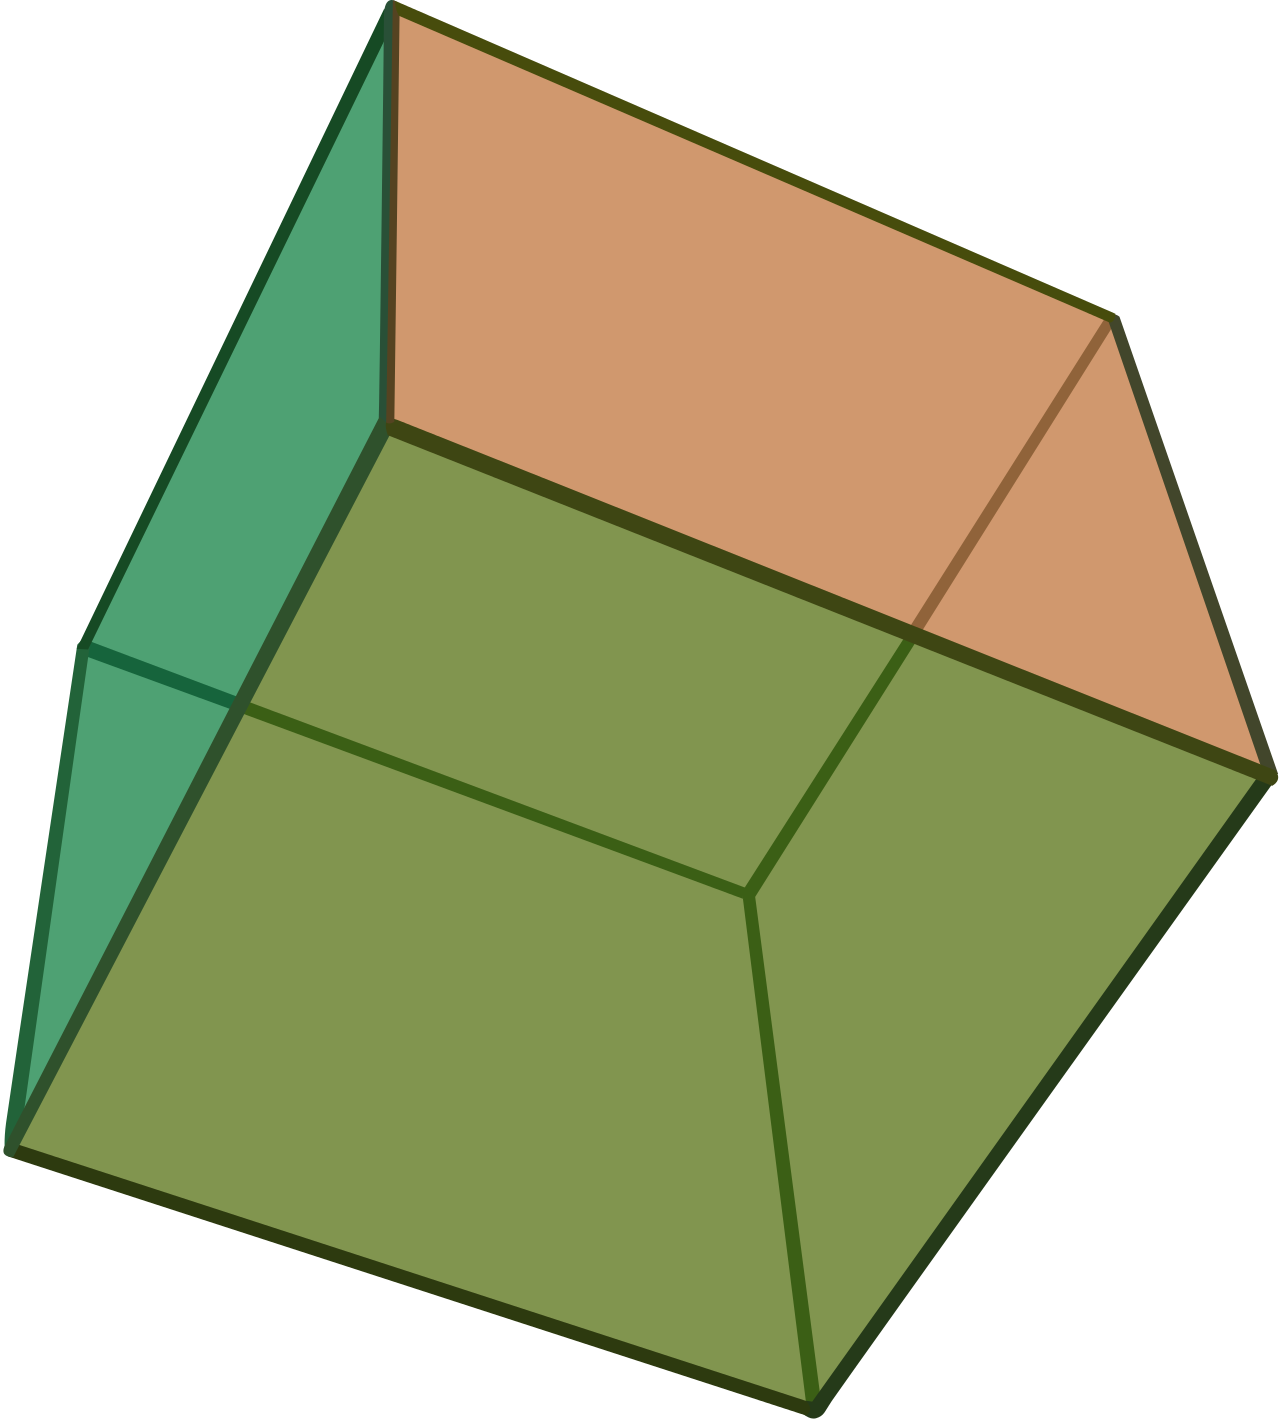
\includegraphics[height = 6cm]{img/Hexahedron.png}
\end{center}

oktaederet,

\begin{center}
    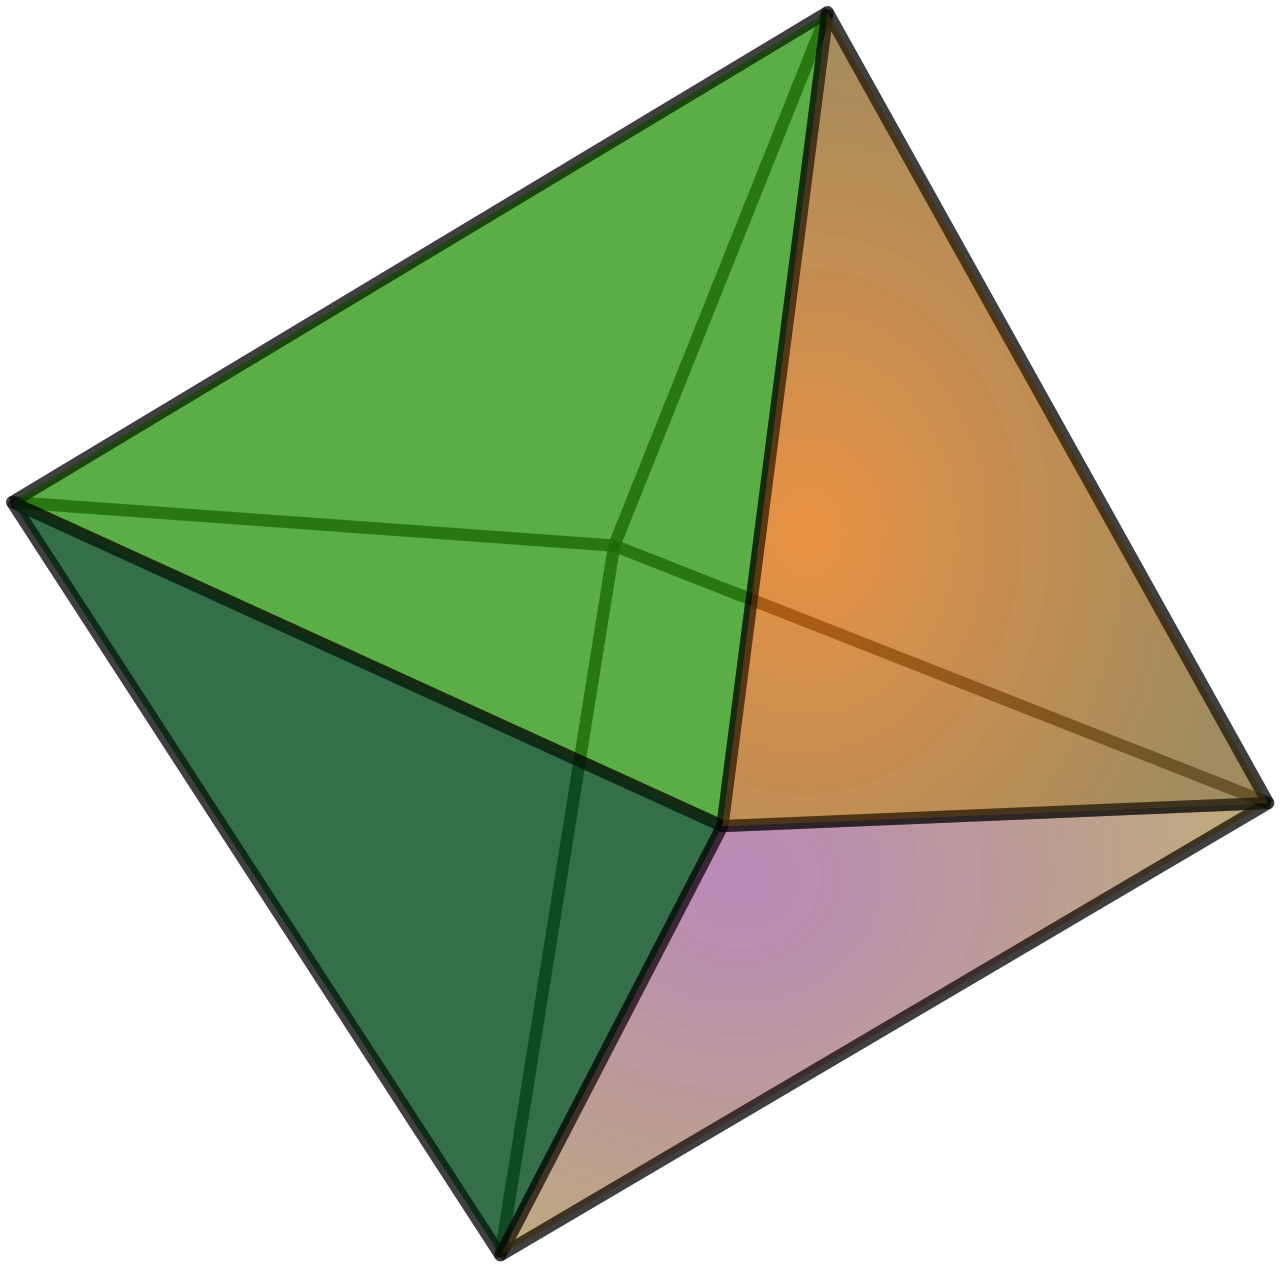
\includegraphics[height = 6cm]{img/Octahedron.png}
\end{center}

dodekaederet,

\begin{center}
    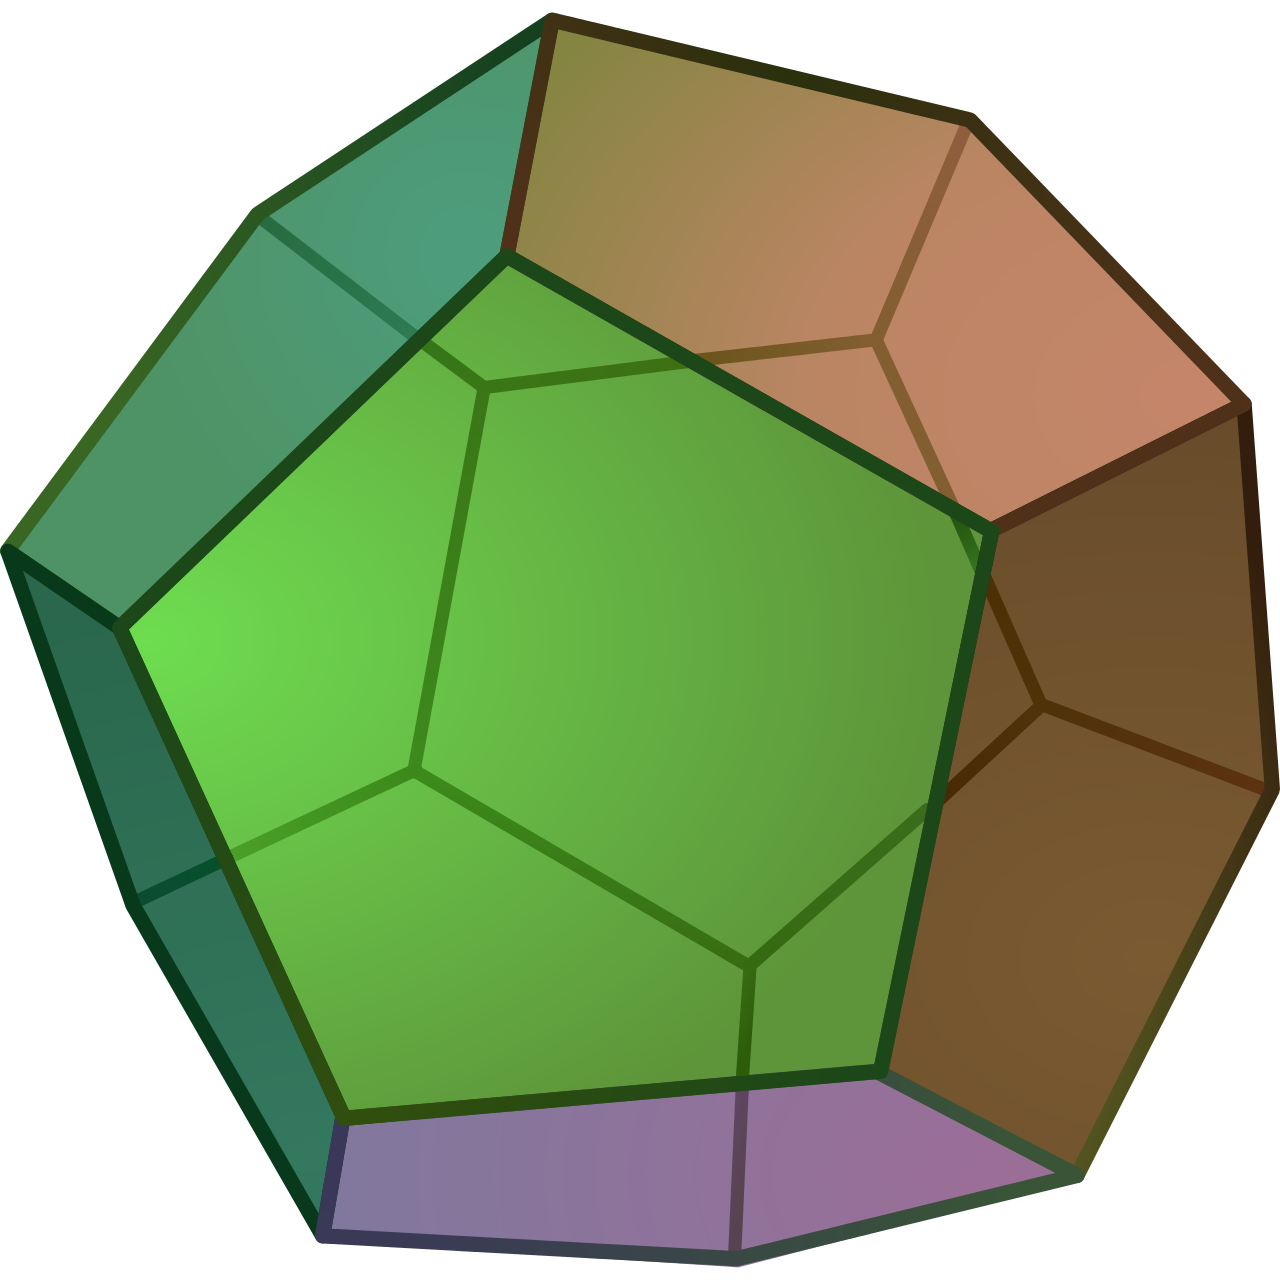
\includegraphics[height = 6cm]{img/Dodecahedron.png}
\end{center}

og til slutt ikosaederet, 

\begin{center}
    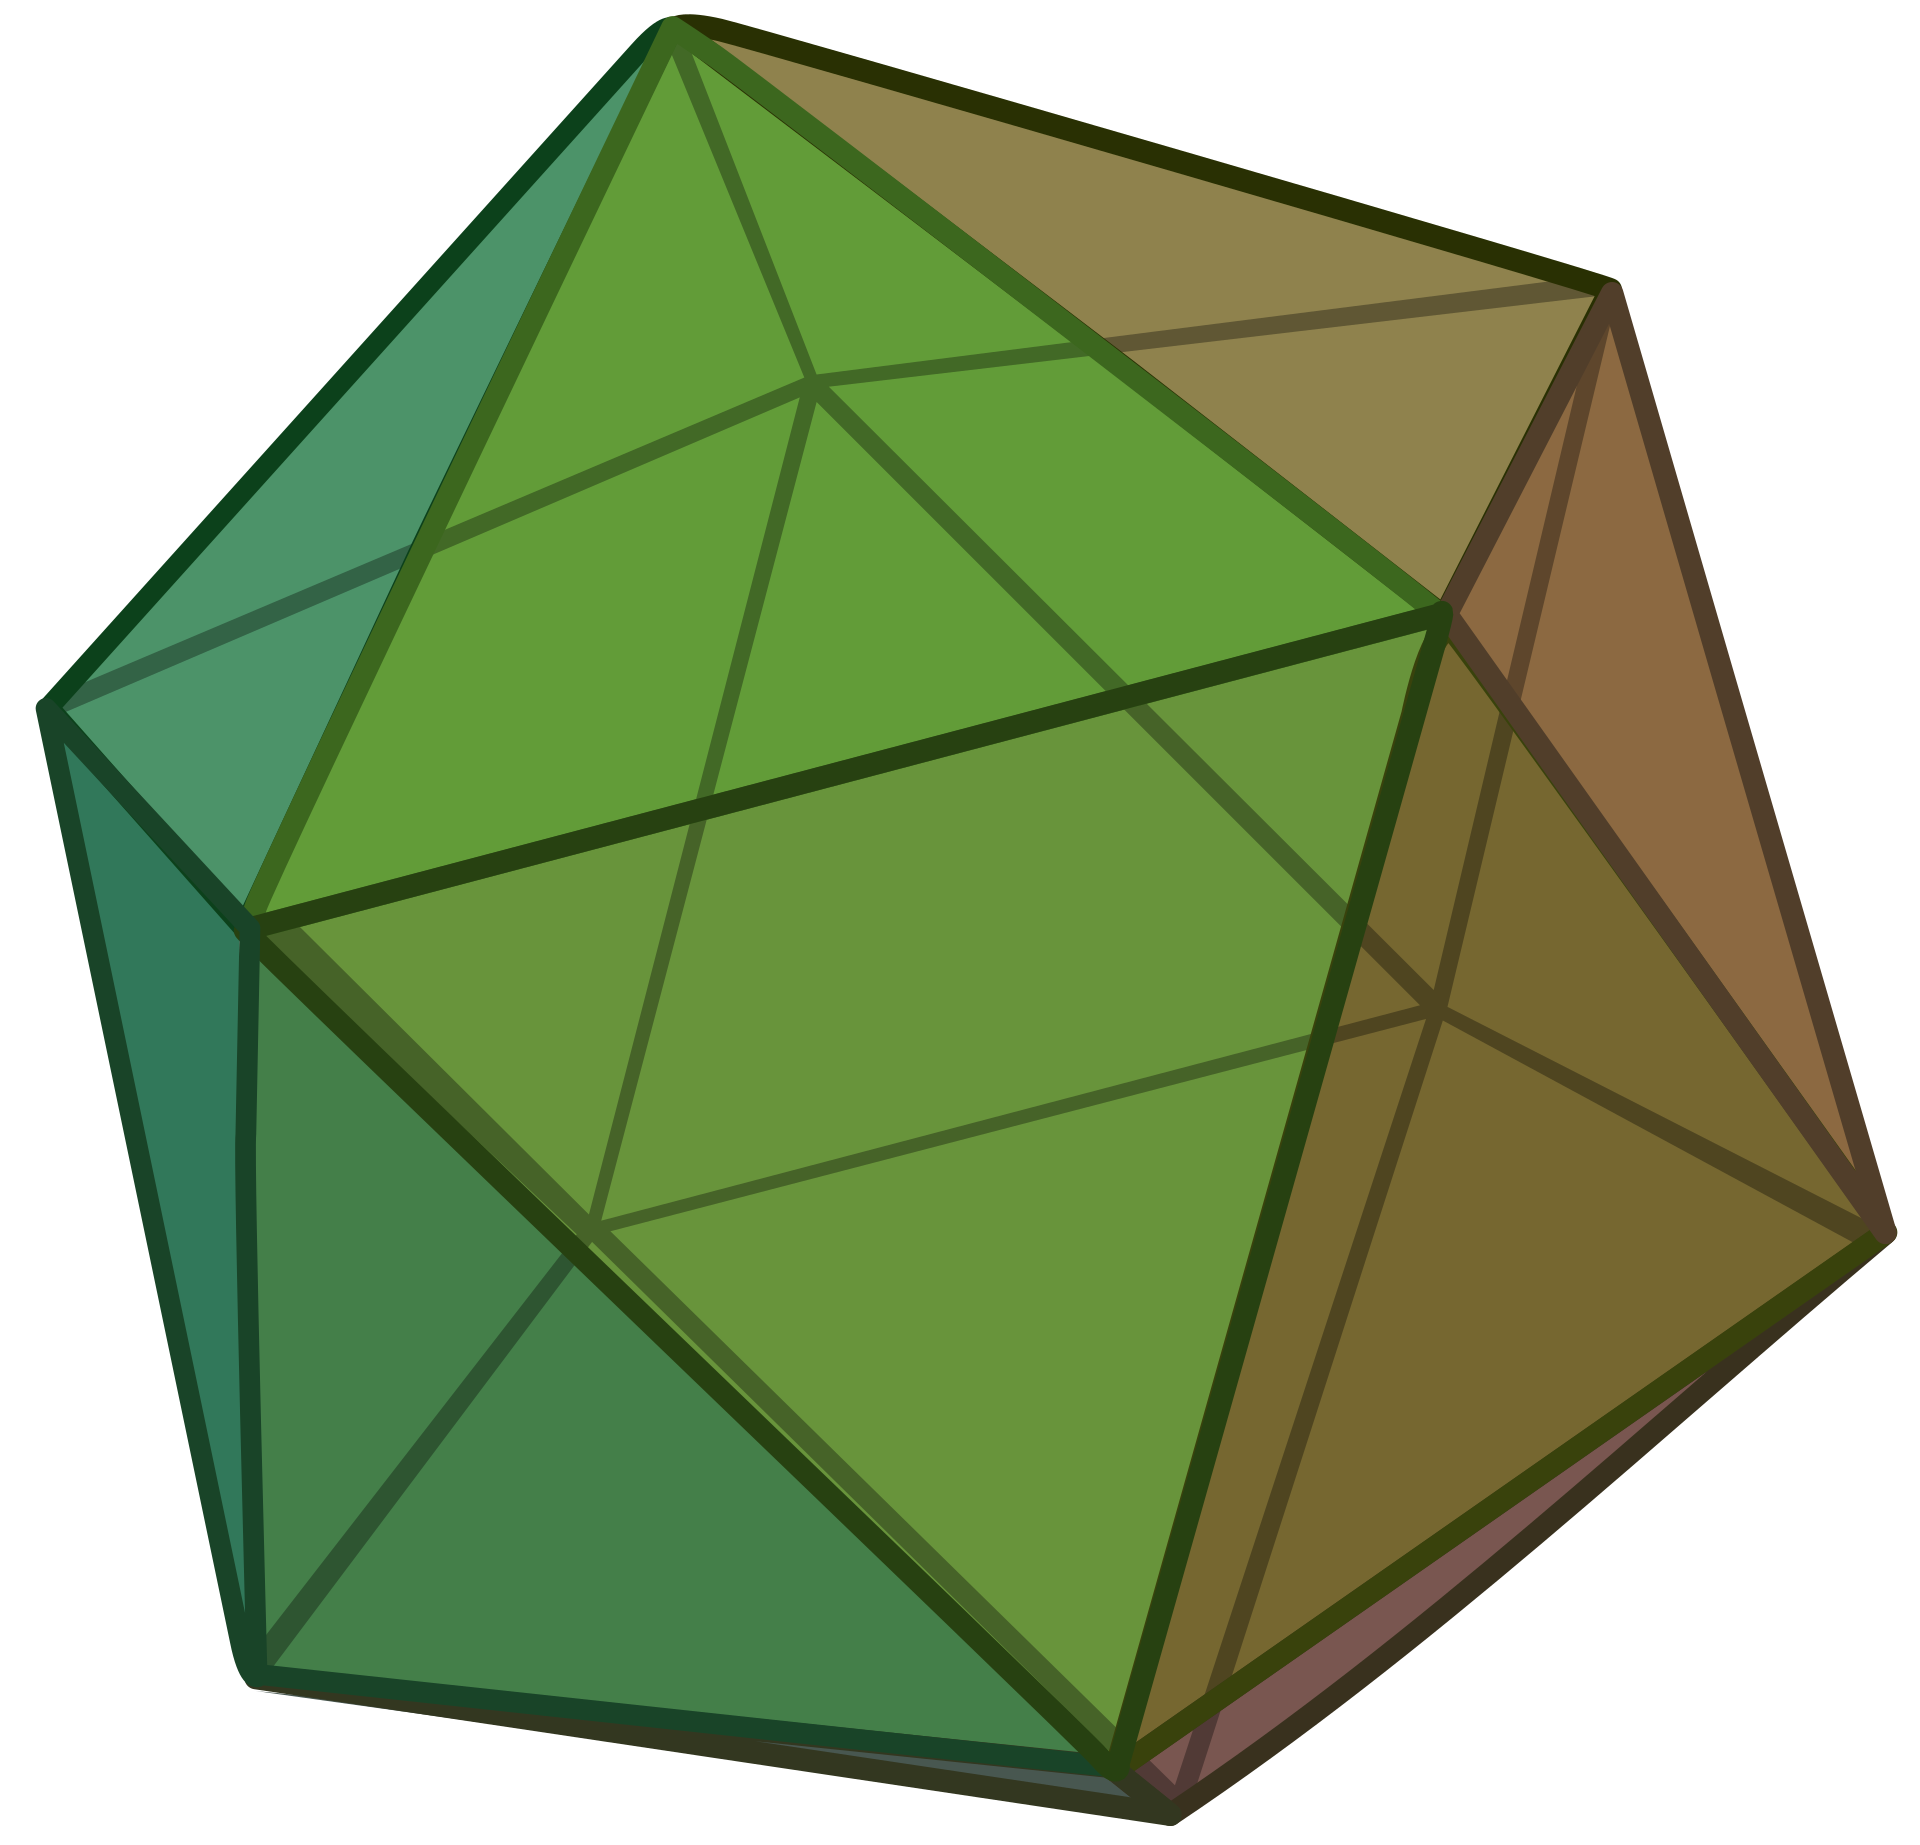
\includegraphics[height = 6cm]{img/Icosahedron.png}
\end{center}

De første tre kan vi beskrive som en trekantet pyramide, en kube og to sammensatte pyramider. Husk disse, de er viktige senere. 

Vi kan lage tilsvarende legemer i alle mulige dimensjoner, ved å sette samme de høyere dimensjonale analogene til polygoner, altså polyhedre. I dimensjon $2$ er det kun linjestykker vi kan sette sammen, så dermed er alle polygoner faktisk Platonske legemer. Vi kan lage polygoner med et vilkårlig antall sidestykker, så det er dermed uendelig antall Platonske legemer i dimensjon $2$. I dimensjon $1$ har vi kun et punkt å bygge disse legemene fra, noe som ikke gir oss mye spillerom. Det er bare et måte å sette sammen et punkt på, som vil si at vi kun har ett Platonsk legeme i dimensjon $1$. 

Det spennende skjer når vi øker dimensjonen over $3$. I dimensjon $4$ har vi litt ekstra rom til å sette sammen figurer, og det er faktisk akkuratt nok rom til å sette sammen et ekstra legeme, så vi har faktisk seks Platonske legemer i dimensjon $4$. Man skulle kanskje tro at dette fenomenet fortsatte i høyere dimensjoner, at man alltid fikk litt mer og mer plass til å lage nye legemer, men dette er faktisk ikke tilfellet. I høyere dimensjoner tar også byggestenene — polyhederene — mer og mer plass, og etter dimensjon $4$ kansellerer disse to effektene hverandre. I alle dimensjoner høyere enn $4$ er det faktisk bare plass til å lage $3$ Platonske legemer! Vi kan alltid lage en høyere dimensjonal kube, en høyere dimensjonal trekantet pyramide, og en høyere dimensjonal versjon av to sammensatte pyramider. 

Så, hvis vi lager en liste med hvor mange Platonske legemer det er i alle dimensjonene får vi 

$$
1,\infty, 5, 6, 3, 3, 3, 3,\ldots
$$

Vi har nå all informasjonen vi trenger til å løse oppgaven. Vi vet at $k=p\cdot q$ der $(p,q)$ er et primtallspar. Vi tester med det første primtallsparet, altså $n=1$, som gir $p=3, q=5$. Da er $k = 15$, men her har vi at $n=1$ ikke er antall Platonske legemer i dimensjon $15$, så dette kan ikke være riktig primtallspar. Vi ser at alle primtallspar vil gi et tall $k$ som er større enn $4$, altså vil alltid antall Platonske legemer i dimensjon $k$ være $3$, uansett hvilket primtallspar vi velger. Dette betyr at $n$ må være lik $3$, som igjen gir at $(p,q) = (11,13)$ ettersom $(11,13)$ er det tredje primtallsparet. Dette gir $k=11\cdot 13 = 143$. Dette tallet gir en gyldig løsning ettersom

\begin{itemize}
    \item $(11,13)$ er et primtallspar
    \item $(11,13)$ er det tredje primtallsparet, altså $n=3$
    \item $n=3$ er antall Platonske legemer i dimensjon $k=11\cdot 13 = 143$
\end{itemize}

Denne løsningen er også unik ettersom alle andre primtallspar vil gi en feil verdi for $n$. Dermed er destinasjonen vår Kjelsåsveien 143, som er adressen til Teknisk museum!


\bibliographystyle{alpha}
\bibliography{references}


\end{document}